
\includegraphics[height=1.5cm]{images/pictograms/tools}


\begin{flushright} {\tiny {\color{gray} python\_codes/fieldstone\_145/text.tex}} \end{flushright}

%\lstinputlisting[language=bash,basicstyle=\small]{python_codes/fieldstone_145/keywords.key}

\begin{center}

\fbox{\textbf{\huge \color{teal} P}}
Code at \url{https://github.com/cedrict/fieldstone/tree/master/python_codes/fieldstone_145}
\end{center}

\par\noindent\rule{\textwidth}{0.4pt}

{\sl This stone was developed in collaboration with Frederic Gueydan}. \index{contributors}{F. Gueydan}

\par\noindent\rule{\textwidth}{0.4pt}
%%%%%%%%%%%%%%%%%%%%%%%%%%%%%%%%%%%%%%%%%%%%%%%%%%%%%%%%%%%%%%%%%%%%%%%%%%%%%%%%%%%%%%%%%%%%%%

This \stone is a simple example of how one can easily read in (p)vtu files, extract the raw data for the fields and 
then for example post-process them, or plot them in a different way.
I cannot predict your exact requirements when it comes to colorscale, aspect ratio, legends, types of data, etc ...
so you will need to figure a few things out on your own. 

In this example there are 4 {\tt .pvtu} files coming from an article in prep. 
These are read in, and converted to png in a crude way. 
This is what the code displays when running
\begin{verbatim}
found  4  pvtu files
processing  solution-00000.pvtu which contains  22905  data points
-----> strain rate m/M: 8.305214e-12 1.1551771e-11
-----> viscosity m/M: 1.8379192e+18 3.4957697e+18
processing  solution-00002.pvtu which contains  22905  data points
-----> strain rate m/M: 5.3416676e-12 1.4275901e-11
-----> viscosity m/M: 1.4940624e+18 6.7333757e+18
processing  solution-00001.pvtu which contains  22905  data points
-----> strain rate m/M: 7.17326e-12 1.27030435e-11
-----> viscosity m/M: 1.6681961e+18 4.2696392e+18
processing  solution-00003.pvtu which contains  22905  data points
-----> strain rate m/M: 3.2133198e-12 1.5906169e-11
-----> viscosity m/M: 1.3733053e+18 2.1652515e+19
\end{verbatim} 
and here are the files produced
\begin{center}
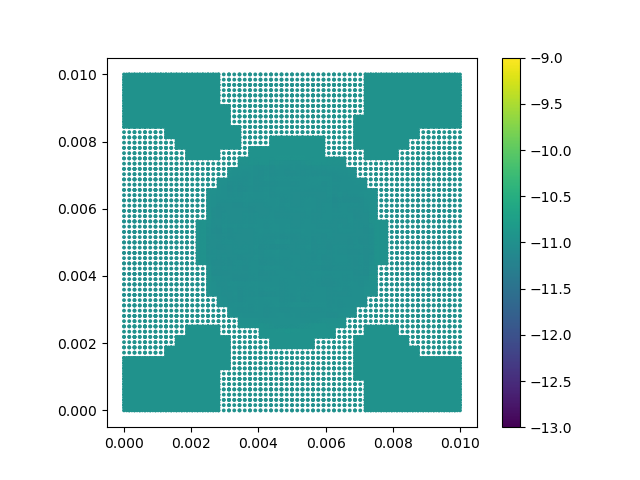
\includegraphics[width=4cm]{python_codes/fieldstone_145/strainrate_0000.png}
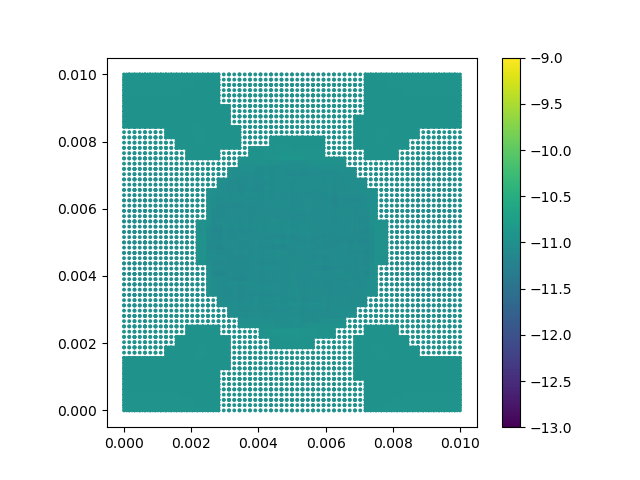
\includegraphics[width=4cm]{python_codes/fieldstone_145/strainrate_0001.png}
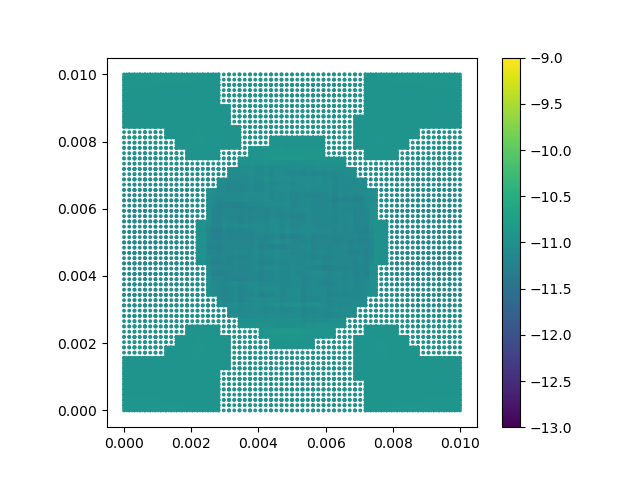
\includegraphics[width=4cm]{python_codes/fieldstone_145/strainrate_0002.png}
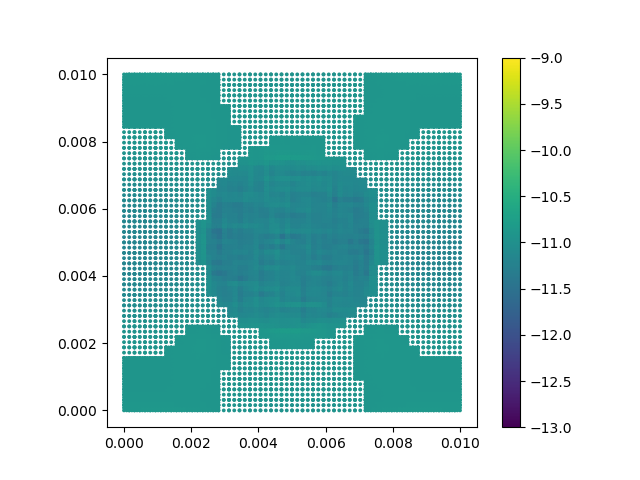
\includegraphics[width=4cm]{python_codes/fieldstone_145/strainrate_0003.png}\\
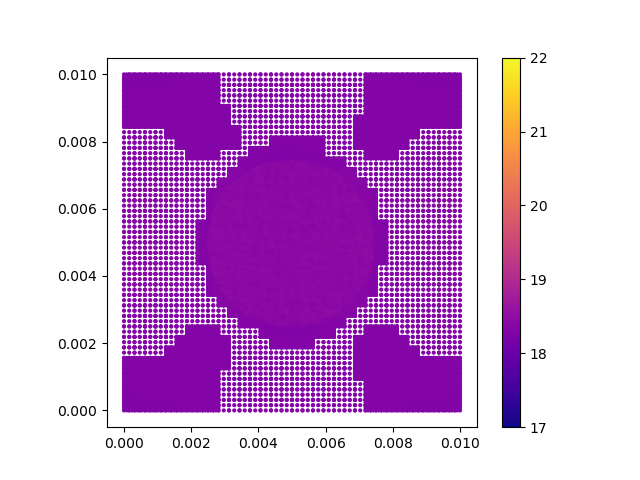
\includegraphics[width=4cm]{python_codes/fieldstone_145/viscosity_0000.png}
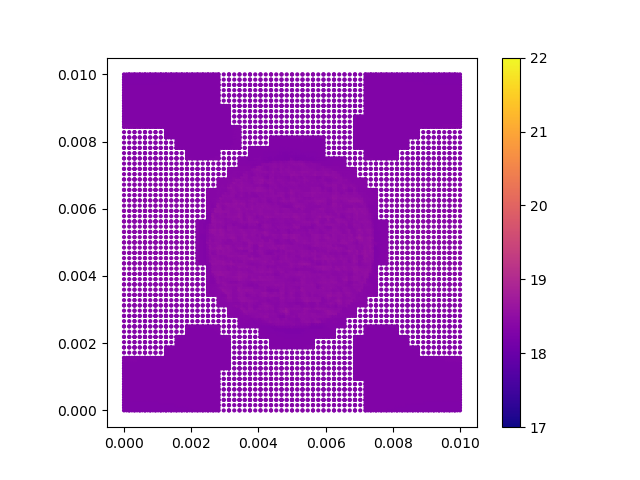
\includegraphics[width=4cm]{python_codes/fieldstone_145/viscosity_0001.png}
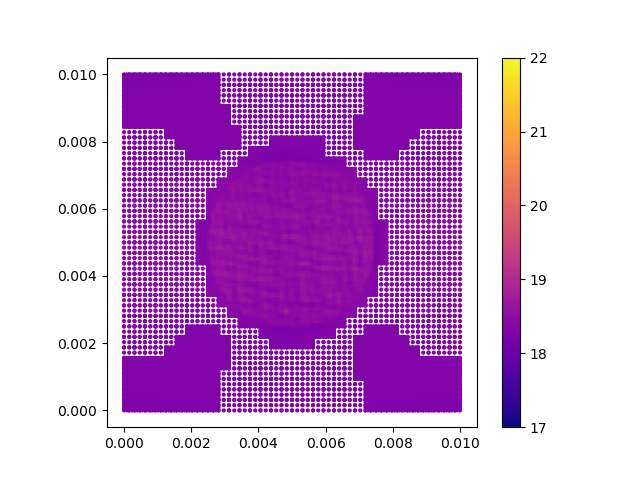
\includegraphics[width=4cm]{python_codes/fieldstone_145/viscosity_0002.png}
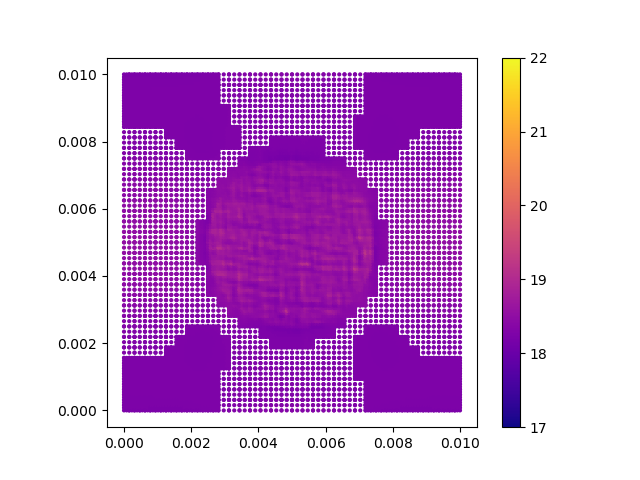
\includegraphics[width=4cm]{python_codes/fieldstone_145/viscosity_0003.png}
\end{center}
 as well as 4 ascii files.

